%% paper.tex
%% IEEE conference paper: Path-Aware Positional Encoding for
%% Raster-Scan Autoregressive Image Generation in CRT Signal Space
%%
%% Compile with: pdflatex paper && bibtex paper && pdflatex paper && pdflatex paper
%% Or: latexmk -pdf paper

\documentclass[conference]{IEEEtran}
\IEEEoverridecommandlockouts

% --- core formatting / typography ---
\usepackage[T1]{fontenc}
\usepackage[utf8]{inputenc}
\usepackage{microtype}      % subtle but real spacing improvements

% --- math / units / numbers ---
\usepackage{amsmath,amssymb,amsfonts}
\usepackage{mathtools}
\usepackage{siunitx}
\sisetup{
  separate-uncertainty,
  detect-weight=true,
  detect-family=true,
  detect-shape=true,
  table-number-alignment=center,
}

% --- tables ---
\usepackage{booktabs}
\usepackage{multirow}
\usepackage{threeparttable}

% --- graphics / figures ---
\usepackage{graphicx}
\usepackage{tikz}
\usetikzlibrary{positioning,arrows.meta,fit,backgrounds,calc,shapes.geometric}
\usepackage{pgfplots}
\pgfplotsset{compat=1.18}

% --- references / cross-refs ---
\usepackage{url}
\usepackage[hidelinks]{hyperref}
\usepackage[capitalize]{cleveref}

% --- algorithms (used in method section) ---
\usepackage{algorithm}
\usepackage[noend]{algpseudocode}

% --- code listings (used to show config) ---
\usepackage{xcolor}
\definecolor{codegray}{gray}{0.95}
\definecolor{codeblue}{rgb}{0.13,0.13,0.5}
\definecolor{codegreen}{rgb}{0,0.5,0}

% Avoid bad hyphenation in technical terms
\hyphenation{Pixel-CNN Pixel-RNN auto-regressive raster-scan}

% =====================================================================
\begin{document}

\title{Path-Aware Positional Encoding for Raster-Scan\\
Autoregressive Image Generation in CRT Signal Space}

\author{
\IEEEauthorblockN{Omar Tweg}
\IEEEauthorblockA{Independent Researcher \\
MechaML, CEO and Founder\\
Cairo, Egypt}
\and
\IEEEauthorblockN{Assem ElQersh}
\IEEEauthorblockA{Independent Researcher \\
MechaML, Head of Deep Learning Team\\
Alexandria, Egypt \\
Email: assem.elqersh.eg@ieee.org}
}

\maketitle

% =====================================================================
\begin{abstract}
We study autoregressive image generation in a 1D \emph{signal space}
obtained by following a CRT-inspired raster-scan path with a
differentiable Gaussian-beam renderer. Within this framing, the
sequence position of a sample and its 2D spatial position on the
screen are not independent: the path is a deterministic, one-to-one
function of the sequence index. We show empirically that, given a
sinusoidal 2D path positional encoding, adding the standard 1D
sequence positional encoding consistently \emph{harms} test
likelihood. On Oxford Flowers~102 at $32\times32$, removing the
sequence encoding improves test bits-per-pixel from
\num{7.16(6)} to \num{6.43(18)} across three seeds at 30~epochs
(Welch $t=5.4$). We also provide multi-seed results for all four
positional-encoding configurations, finding that the sequence
encoding alone (without path) yields $7.12\pm0.11$ bpd, nearly
identical to the full model, while removing both encodings
degrades performance to $9.03\pm0.01$ bpd, confirming that the
path encoding is the informative component. The direction of the
effect is preserved in a three-seed comparison at $48\times48$
(Welch $t=-1.97$, 15~epochs).
Extending this analysis at a matched sequence length
($N{=}1024$, single-sample-per-pixel raster), we find that
\emph{traversal locality} -- the mean sequence distance between
four-neighbour pixel pairs -- predicts test bpd with Pearson
$r=0.996$ ($p<10^{-4}$, $n=9$) across four hand-designed
traversals and five random pixel permutations, identifying
1D serialisation of 2D structure as the architectural
bottleneck rather than the specific scan order. Four
architectural probes (delta input encoding, patch-hierarchical
traversal, epoch-level traversal augmentation, and a causal 1D
conv-stem) all fail to improve over the matched-$N$ raster
baseline, suggesting the remaining gap to pixel-space methods
requires genuinely 2D-aware computation rather than
surface-level re-orderings or shallow 1D inductive bias.
We additionally test
three CRT-physics-motivated architectural modifications
(learned per-step beam focus, phosphor persistence, and learned
beam-position perturbation) against the same baseline at three seeds;
none reaches statistical significance ($|t|<1$). A matched-parameter
PixelCNN++ trained under the same protocol attains a stronger
absolute likelihood ($\SI{4.71(2)}{}$ bpd at 30 epochs), so the
observed encoding effect is best read as architecture-specific to
signal-space autoregressive models rather than a closure of the
gap to pixel-space methods.
\end{abstract}

\begin{IEEEkeywords}
autoregressive models, image generation, positional encoding,
likelihood, ablation
\end{IEEEkeywords}

% =====================================================================
\section{Introduction}

Autoregressive image models factor a joint distribution
$p(\mathbf{x})$ over an image $\mathbf{x}$ as a product of conditional
distributions over a chosen ordering of its components. PixelRNN and
PixelCNN~\cite{vandenoord2016pixelrnn} introduced the now-standard
choice of a row-major raster scan over pixels, and subsequent work
\cite{salimans2017pixelcnnpp,parmar2018imagetransformer,chen2020generative}
has retained that ordering while replacing the underlying architecture.
Within this lineage, position information is uniformly encoded by
the position in the 1D sequence, which is identified with the
position in the 2D image through the implicit raster mapping.

A separate body of work~\cite{ha2017sketchrnn,
ganin2018spiral,liu2021painttransformer,frans2021clipdraw,jain2023vectorfusion}
treats image synthesis as the production of a continuous trajectory
that is then deposited onto a canvas by a (typically differentiable)
renderer. The model never directly emits pixel intensities; it emits
control signals for an external rendering process. We refer to this
family as \emph{signal-space} generative modelling.

The two framings can be unified by adopting an \emph{intermediate}
representation: the model emits a 1D sequence of intensities sampled
along a deterministic raster-scan path, and a Gaussian-beam renderer
deposits those intensities onto a 2D grid. This formulation makes
explicit a property that is implicit in PixelRNN-style models: each
1D sequence position carries an associated 2D path coordinate, and
the mapping between them is invertible. As a result, the modeller
has two natural choices for positional encoding, the 1D sequence
index and the 2D path coordinate, which are individually unsurprising
but \emph{redundant} when used together.

This paper studies the consequences of that redundancy. We find
that it is not benign: at matched parameters and training budget,
adding the 1D sequence encoding to a model that already has a 2D
path encoding makes test likelihood reliably worse. We verify this
with multi-seed ablations at two image sizes, examine three
CRT-physics--motivated architectural modifications as additional
ablation targets, and benchmark against a matched-parameter
PixelCNN++ to place the absolute numbers in context.

\paragraph{Contributions.}
\begin{enumerate}
  \item We formalise the redundancy between sequence and path
    positional encodings in raster-scan signal-space autoregressive
    models, and show that adding the sequence encoding to a model
    that already has the path encoding hurts likelihood by
    \SI{0.73(19)}{} bpd
    on Oxford Flowers at $32\times32$ ($t=5.4$, 3~seeds, 30~epochs).
    We additionally provide all four positional-encoding
    configurations at three seeds, confirming that the path encoding
    is the informative component. The direction of the effect
    persists at $48\times48$ (Welch $t=-1.97$, 3~seeds, 15~epochs).
  \item We test three CRT-physics--motivated modifications
    (learned beam focus, phosphor persistence, beam-position
    perturbation) under the same protocol as a falsifiability check
    on the broader ``CRT-inspired'' framing. None reaches statistical
    significance ($|t|<1$, three seeds each).
  \item We provide a matched-parameter PixelCNN++ baseline under
    identical conditioning, training, and evaluation, allowing a
    direct comparison between signal-space and pixel-space
    autoregressive models on the same data.
  \item We show that traversal locality predicts test bpd with
    Pearson $r=0.996$ ($p<10^{-4}$) across four hand-designed
    traversals and five random pixel permutations at matched
    $N{=}1024$, localising the bottleneck in serialised image AR
    to 1D-serialisation of 2D-neighbour structure rather than
    scan-order choice.
  \item We test four architectural probes (delta input encoding,
    patch-hierarchical traversal, traversal augmentation, causal
    1D conv-stem) against the matched-$N$ raster baseline; none
    improves over baseline, narrowing the design space for future
    work to 2D-aware computational blocks.
\end{enumerate}

% =====================================================================
\section{Related Work}\label{sec:related}

\paragraph{Autoregressive image models.}
PixelRNN/PixelCNN \cite{vandenoord2016pixelrnn} established raster-order
factorisation as the dominant approach. PixelCNN++
\cite{salimans2017pixelcnnpp} introduced the discretised mixture-of-logistics
(DMoL) output distribution and several other refinements; we adopt the
DMoL head verbatim. Image Transformer~\cite{parmar2018imagetransformer}
and iGPT~\cite{chen2020generative} replace masked convolutions with
self-attention while keeping the raster ordering. Recent work has
revisited the ordering choice itself: RadAR~\cite{li2025radar} uses
a radial scan, and \cite{li2025direction} explores diagonal orderings,
both reporting that raster order remains a strong default. None of
these works isolates the role of the 1D sequence positional
encoding given an additional 2D path encoding.

\paragraph{Stroke- and trajectory-based generation.}
SketchRNN~\cite{ha2017sketchrnn} models pen trajectories with an RNN.
SPIRAL~\cite{ganin2018spiral} learns a painting agent through
reinforcement learning against a differentiable renderer. Paint
Transformer~\cite{liu2021painttransformer} predicts strokes
feed-forward. CLIPDraw~\cite{frans2021clipdraw} and
VectorFusion~\cite{jain2023vectorfusion} optimise SVG strokes using
CLIP-based objectives. Our renderer is closest in spirit to the
DiffVG~\cite{li2020diffvg} family but specialised to a raster
scan with finite beam width.

\paragraph{Differentiable rasterisation.}
The 2D Gaussian splatting view has a long history; a recent
high-profile incarnation is 3D Gaussian splatting
\cite{kerbl20233dgaussian}. Our 2D variant is a special case with
deterministic, fixed splat positions and a learnable (in V6 ablation)
or fixed (default) beam width.

% =====================================================================
\section{Method}\label{sec:method}

We describe the signal-space framing
(\cref{ssec:framing}), the architecture used to predict the signal
(\cref{ssec:arch}), and the differentiable renderer that maps the
signal back to a 2D image (\cref{ssec:renderer}). We then define
the four positional-encoding configurations that are the central
object of study (\cref{ssec:pe}).

\subsection{Signal-Space Framing}\label{ssec:framing}

Let $\mathbf{x}\in[0,1]^{C\times H\times W}$ be a target image. We
fix a deterministic raster path
$\mathcal{P}=(\mathbf{p}_1,\ldots,\mathbf{p}_N)$ with
$\mathbf{p}_i=(x_i,y_i)\in\mathbb{R}^2$ that traverses the image row
by row at $r$ samples per pixel, with a fraction $f$ of every row
allocated to a non-emitting flyback segment from the right edge
back to the left edge. Each sample is assigned a binary mask
$m_i\in\{0,1\}$ with $m_i=1$ on the active row sweep and $m_i=0$
during flyback. For Oxford Flowers at $32\times32$ with $r=2$ and
$f=0.08$ this yields $N=2208$ and $\sum_i m_i / N \approx 0.928$.

The target signal $\mathbf{s}\in[0,1]^{N\times C}$ is obtained by
bilinearly sampling $\mathbf{x}$ at each path position:
\begin{equation}
  \mathbf{s}_i = m_i \cdot \mathrm{Bilinear}(\mathbf{x},\mathbf{p}_i).
\end{equation}
We model the joint distribution
$p_\theta(\mathbf{s}\mid\mathbf{c})$, where $\mathbf{c}$ is a CLIP
ViT-B/32 text embedding of a class-template caption such as
``a photo of a [class name].''

\subsection{Architecture}\label{ssec:arch}

The architecture (Fig.~\ref{fig:arch}) is a six-block causal
transformer with FiLM~\cite{perez2018film} conditioning on the CLIP
embedding and a DMoL output head with $K=5$ mixture components.
We use \textbf{$d_{\text{model}}=256$, $n_{\text{heads}}=4$},
feed-forward expansion factor $4$, and dropout $0.1$. The full model
contains \num{6520867} trainable parameters.

% fig_arch.tex
% Architecture diagram. Compact horizontal layout:
% (LEFT)  conditioning chain     -> FiLM input to transformer
% (CENTRE) data flow column      -> shifted input -> transformer -> head
% (RIGHT) inference render chain -> sample -> renderer -> output

\begin{figure}[t]
\centering
\resizebox{\columnwidth}{!}{%
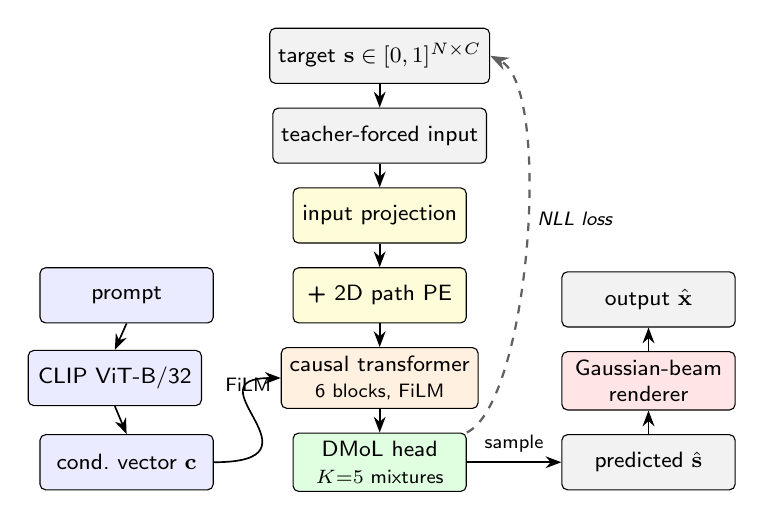
\begin{tikzpicture}[
    font=\sffamily\footnotesize,
    >=Stealth,
    node distance=3mm,
    box/.style    ={draw, rounded corners=2pt, inner sep=3pt,
                    minimum height=7mm, minimum width=22mm,
                    align=center, fill=white},
    txtbox/.style ={box, fill=blue!8},
    netbox/.style ={box, fill=orange!12},
    headbox/.style={box, fill=green!12},
    rendbox/.style={box, fill=red!10},
    inbox/.style  ={box, fill=gray!10},
    arr/.style={->, semithick},
]

% =========================================================
% Centre column: data flow (top -> bottom)
% =========================================================
\node[inbox]              (sig)   {target $\mathbf{s}\in[0,1]^{N\times C}$};
\node[inbox, below=of sig](input) {teacher-forced input};
\node[box,   fill=yellow!15, below=of input] (proj)
        {input projection};
\node[box,   fill=yellow!15, below=of proj] (pe)
        {{\bfseries +} 2D path PE};

% Transformer (visual stack)
\begin{scope}[on background layer]
\node[netbox, below=of pe, xshift=0.7mm, yshift=-0.7mm] (b2) {};
\end{scope}
\node[netbox, below=of pe] (tx)
    {causal transformer\\\scriptsize 6 blocks, FiLM};

\node[headbox, below=of tx] (head)
    {DMoL head\\\scriptsize $K{=}5$ mixtures};

% Centre arrows
\draw[arr] (sig.south)   -- (input.north);
\draw[arr] (input.south) -- (proj.north);
\draw[arr] (proj.south)  -- (pe.north);
\draw[arr] (pe.south)    -- (tx.north);
\draw[arr] (tx.south)    -- (head.north);

% =========================================================
% Left column: conditioning, aligned with transformer
% =========================================================
\node[txtbox, left=10mm of pe.west,  anchor=east] (txt)  {prompt};
\node[txtbox, left=10mm of tx.west,  anchor=east] (clip) {CLIP ViT-B/32};
\node[txtbox, left=10mm of head.west,anchor=east] (cond) {cond.\ vector $\mathbf{c}$};
\draw[arr] (txt.south)  -- (clip.north);
\draw[arr] (clip.south) -- (cond.north);

% Conditioning -> transformer (FiLM)
\draw[arr] (cond.east) .. controls +(15mm,0) and +(-12mm,0) ..
    node[pos=0.65, above, font=\sffamily\scriptsize]{FiLM}
    (tx.west);

% =========================================================
% Right column: inference rendering chain
% =========================================================
\node[inbox,   right=12mm of head, anchor=west] (pred)
    {predicted $\hat{\mathbf{s}}$};
\node[rendbox, above=of pred] (rend)
    {Gaussian-beam\\renderer};
\node[inbox, above=of rend] (out)
    {output $\hat{\mathbf{x}}$};

\draw[arr] (head.east) -- node[above, font=\sffamily\scriptsize]{sample}
    (pred.west);
\draw[arr] (pred.north) -- (rend.south);
\draw[arr] (rend.north) -- (out.south);

% =========================================================
% Training loss (dashed): head -> target signal
% =========================================================
\draw[arr, dashed, gray!75!black, thick]
    (head.north east) .. controls +(8mm,4mm) and +(8mm,-4mm) ..
    node[pos=0.55, right, font=\sffamily\scriptsize\itshape, black]
        {NLL loss}
    (sig.east);

\end{tikzpicture}%
}
\caption{Signal-space autoregressive architecture. The target image
is converted to a 1D signal $\mathbf{s}$ by sampling along a fixed
raster path (omitted from the figure for clarity). A causal
transformer with FiLM conditioning on a CLIP text embedding
$\mathbf{c}$ predicts the next signal value at each step. The DMoL
output head provides the training likelihood (dashed arrow back to
the target). At inference, the predicted signal $\hat{\mathbf{s}}$
is mapped to an image $\hat{\mathbf{x}}$ by the differentiable
Gaussian-beam renderer (right column).}
\label{fig:arch}
\end{figure}


For each step $i$ the head emits parameters of an RGB-factorised
mixture of logistics. We compute the negative log-likelihood
$\mathrm{NLL}(\mathbf{s})$ of the discretised target (256 bins per
channel) and average over active positions:
\begin{equation}
  \mathcal{L}(\theta) = \frac{\sum_i m_i \, \mathrm{NLL}_\theta(\mathbf{s}_i)}{\sum_i m_i}.
\end{equation}
Following \cite{salimans2017pixelcnnpp} we train with teacher forcing,
adding scheduled sampling~\cite{bengio2015scheduled} at probability
$p_{\text{ss}}$ linearly ramped from 0 to $0.25$ across training to
mitigate exposure bias on long sequences.

\subsection{Differentiable Renderer}\label{ssec:renderer}

The renderer maps a predicted signal $\hat{\mathbf{s}}$ to a 2D image
$\hat{\mathbf{x}}\in[0,1]^{C\times H\times W}$ by depositing each
sample as a 2D Gaussian at its path position with width $\sigma$:
\begin{equation}
  \hat{\mathbf{x}}_{c,h,w} = \frac{1}{Z}\sum_{i=1}^N m_i \, \hat{\mathbf{s}}_{i,c} \,
    \exp\!\left(-\frac{(h-y_i)^2 + (w-x_i)^2}{2\sigma^2}\right),
\end{equation}
where $Z = r \cdot 2\pi\sigma^2$ is a fixed normalisation tied to
the kernel integral and the active-sample density. Unlike
per-image max normalisation, this is smooth in the gradient and
preserves a linear correspondence between signal magnitude and
image brightness. We use $\sigma=0.75$ throughout the main
results.

\subsection{Positional Encodings}\label{ssec:pe}

The encoder optionally adds, at each step, two sinusoidal
embeddings:

\paragraph{1D sequence encoding $\mathbf{e}^{\text{seq}}_i$.}
The standard~\cite{vaswani2017attention} sinusoidal embedding
indexed by $i\in\{1,\ldots,N\}$.

\paragraph{2D path encoding $\mathbf{e}^{\text{path}}_i$.}
A 2D sinusoidal embedding of the continuous coordinate
$\mathbf{p}_i=(x_i,y_i)$, normalised to $[0,1]$. Half of the
$d_{\text{model}}$ channels encode $x_i$, the other half $y_i$.

We study four configurations: \textbf{both} (sequence + path),
\textbf{seq~only}, \textbf{path~only}, and \textbf{neither}.
Because the path is deterministic, $\mathbf{e}^{\text{path}}_i$
is recoverable from $\mathbf{e}^{\text{seq}}_i$ by composition with
$\mathcal{P}$. The two encodings are therefore informationally
redundant when used together: the question is whether their
\emph{form} hurts optimisation.

% =====================================================================
\section{Experiments}\label{sec:experiments}

\subsection{Setup}

\paragraph{Dataset.}
Oxford Flowers~102~\cite{nilsback2008flowers} (\num{7169} train /
\num{1020} test images, all resized to $32\times32$ for the main
experiments and $48\times48$ for the scaling study).

\paragraph{Training.}
AdamW~\cite{loshchilov2019adamw} ($\beta_1=0.9$, $\beta_2=0.95$,
weight decay $10^{-2}$) with peak learning rate $3\!\times\!10^{-4}$,
linear warmup over 500~steps and cosine decay to zero.
Gradient clipping at norm 1.0. Mixed-precision training (fp16) on a
single NVIDIA T4 GPU.

\paragraph{Evaluation.}
We report \emph{bits-per-pixel} (bpd) under the same convention as
PixelCNN++~\cite{salimans2017pixelcnnpp}:
\begin{equation}\label{eq:bpd}
  \text{bpd} = \frac{1}{H\,W\,C\,\ln 2}\,\mathbb{E}_{\mathbf{x}}\!\left[
    -\log p_\theta(\mathbf{x}\mid\mathbf{c})\right].
\end{equation}
Note that for the signal-space model the per-image NLL is the sum
over all active signal positions, but the divisor in
\cref{eq:bpd} is $H\,W\,C$ (the number of sub-pixels), \emph{not}
the number of signal samples; this keeps the unit comparable across
architectures.

\subsection{Main Result: Sequence vs.\ Path Encoding}\label{ssec:main}

We compare the four positional-encoding configurations of
\cref{ssec:pe} on the held-out test split. \Cref{tab:main} reports
mean and standard deviation across three seeds at 30~epochs.

\begin{table}[t]
\centering
\caption{Test bits-per-pixel and per-image NLL on Oxford Flowers
$32\times32$, 30~epochs, 3~seeds (seeds 0--2). Lower is better.}
\label{tab:main}
\begin{tabular}{l S[table-format=5.1(4)] S[table-format=1.3(3)]}
\toprule
Configuration & {NLL (nats/img)} & {bpd} \\
\midrule
seq + path (full)    & 15249.9(1185) & 7.156(56)  \\
seq only             & 15158.0(2365) & 7.119(111) \\
\textbf{path only}   & \bfseries 13695.9(3898) & \bfseries 6.432(183) \\
neither              & 19227.0(159)  & 9.030(7)   \\
\bottomrule
\end{tabular}
\end{table}

With all four configurations now measured at three seeds, the
bpd hierarchy is: \textbf{path only} ($6.43 \pm 0.18$)
$<$ \textbf{seq only} ($7.12 \pm 0.11$)
$\approx$ \textbf{full} ($7.16 \pm 0.06$)
$\ll$ \textbf{neither} ($9.03 \pm 0.01$).
Two results stand out. First, the path-only configuration improves
over full by \num{1554} nats/image (\SI{0.73}{} bpd); the pooled
standard error is $\sqrt{(118.5^2+389.8^2)/3}=\num{235.5}$ nats,
giving $t=\num{6.6}$ (Welch $t=\num{5.4}$), a robust finding.
Second, the absence of any encoding (``neither'') degrades
performance drastically by \SI{2.60}{} bpd relative to path-only,
while seq-only alone recovers most of path-only's gain ($7.12$ vs
$9.03$), confirming that the \emph{path} encoding is the
informative component. The near-identical performance of ``full''
and ``seq only'' ($t=-0.60$, not significant) shows that the
sequence encoding adds negligible information beyond what the
path encoding already provides, but does
introduce a small optimisation penalty when both are present.

\paragraph{Convergence study.}
A single-seed 60-epoch run with the path-only configuration shows
that the model continues to improve well past the 30-epoch budget
(\cref{fig:curves}), reaching $\SI{5.24}{}$ bpd at the best
checkpoint (epoch~55).

% fig_curves.tex
% Training curves for the path-only configuration (V5 60-epoch run).
% Data points are taken from the validation log every 5 epochs.

\begin{figure}[t]
\centering
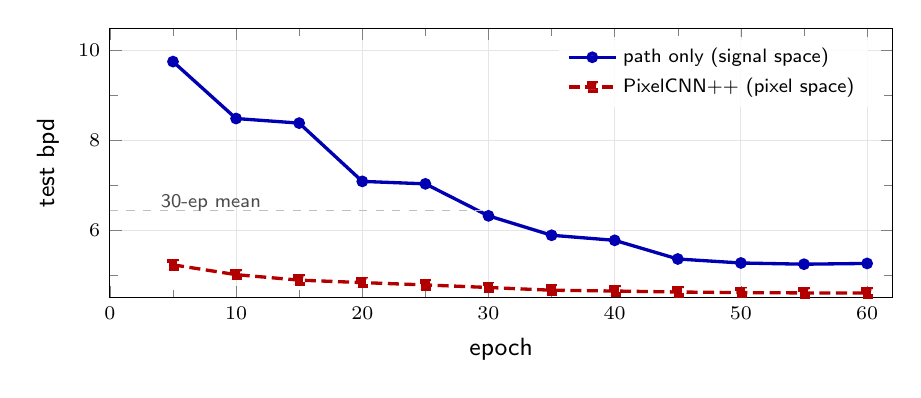
\begin{tikzpicture}
\begin{axis}[
    width=0.95\columnwidth,
    height=5cm,
    xlabel={epoch},
    ylabel={test bpd},
    xmin=0, xmax=62,
    ymin=4.5, ymax=10.5,
    grid=major,
    grid style={gray!20},
    minor tick num=1,
    legend pos=north east,
    legend cell align={left},
    legend style={font=\sffamily\scriptsize, draw=none, fill=white,
                  fill opacity=0.85, text opacity=1},
    label style={font=\sffamily\small},
    tick label style={font=\sffamily\scriptsize},
    every axis plot/.append style={very thick},
]
% V5 path-only (signal-space) -- from 60-epoch run
\addplot[color=blue!70!black, mark=*, mark size=1.5pt] coordinates {
  (5, 9.756) (10, 8.487) (15, 8.385) (20, 7.086) (25, 7.031)
  (30, 6.318) (35, 5.885) (40, 5.772) (45, 5.356) (50, 5.267)
  (55, 5.240) (60, 5.257)
};
\addlegendentry{path only (signal space)}

% PixelCNN++ -- from 60-epoch run
\addplot[color=red!70!black, mark=square*, mark size=1.5pt,
         dash pattern=on 4pt off 2pt] coordinates {
  (5, 5.226) (10, 5.007) (15, 4.885) (20, 4.830) (25, 4.778)
  (30, 4.721) (35, 4.660) (40, 4.642) (45, 4.620) (50, 4.607)
  (55, 4.600) (60, 4.598)
};
\addlegendentry{PixelCNN++ (pixel space)}

% Reference line for V5 30-epoch path-only
\draw[gray!50, dashed] (axis cs:0,6.432) -- (axis cs:30,6.432);
\node[font=\sffamily\scriptsize, gray!60!black] at (axis cs:8,6.6)
    {30-ep mean};

\end{axis}
\end{tikzpicture}
\caption{Validation bits-per-pixel during training. Signal-space
(blue) is the path-only configuration of \cref{ssec:main}; pixel-space
(red, dashed) is the matched-parameter PixelCNN++ baseline of
\cref{ssec:pixelcnn}. Both are single-seed runs over 60 epochs. The
dashed grey line marks the multi-seed mean of the path-only
configuration at 30 epochs ($\SI{6.43}{}$ bpd).}
\label{fig:curves}
\end{figure}


\subsection{Scaling to $48\times48$}\label{ssec:scale}

To check that the encoding effect is not specific to a particular
sequence length, we repeat the comparison at $48\times48$, where
$N=4944$, using three seeds at 15~epochs (\cref{tab:scale}).
The path-only configuration still outperforms the full model on
average by \SI{0.40}{} bpd (Welch $t=-1.97$). The effect is weaker
than at $32\times32$ in statistical terms, mainly because one
path-only seed achieved \SI{8.03}{} bpd while the other two
converged to $\approx 8.64$ bpd, inflating the variance. The sign
of the effect is nonetheless preserved across all three seeds, and
the mean path-only bpd (\num{8.43}) is lower than the mean full bpd
(\num{8.83}) by a consistent margin. We report this as supporting
evidence that the encoding redundancy does not vanish at longer
sequences, while acknowledging the weaker statistical strength at
this scale.

\begin{table}[t]
\centering
\caption{Scaling to $48\times48$: 15~epochs, 3~seeds (seeds 0--2).
The path-only advantage persists with longer sequences
(Welch $t=-1.97$).}
\label{tab:scale}
\begin{tabular}{lcc}
\toprule
Configuration & bpd mean & bpd std \\
\midrule
seq + path (full)        & 8.831 & 0.036 \\
\textbf{path only}       & \bfseries 8.433 & \bfseries 0.348 \\
\midrule
$\Delta$ (path only better by) & 0.398 & \\
Welch $t$                & $-1.97$ & \\
\bottomrule
\end{tabular}
\end{table}

\subsection{Comparison with Pixel-Space PixelCNN++}\label{ssec:pixelcnn}

We re-implement PixelCNN++~\cite{salimans2017pixelcnnpp} with the
same CLIP--FiLM conditioning, the same DMoL head, and matched
parameter count (\num{6417795}, $98.4\%$ of our model). Critically,
the evaluation function is identical: per-image NLL summed over all
pixel positions, divided by $H\,W\,C \ln 2$.

\begin{table}[t]
\centering
\caption{Direct comparison on Oxford Flowers $32\times32$ at matched
parameter count. Multi-seed numbers are mean $\pm$ std across seeds
0--2; single-seed entries use seed 0.}
\label{tab:pixelcnn}
\begin{threeparttable}
\begin{tabular}{l S[table-format=1.2] S[table-format=2.0(0)] S[table-format=1.2(2)]}
\toprule
Model & {Params (M)} & {Epochs} & {bpd (test)} \\
\midrule
\multicolumn{4}{l}{\textit{Signal-space (this work)}} \\
\quad full        & 6.52 & 30  & 7.156(56)  \\
\quad path only   & 6.52 & 30  & 6.432(183) \\
\quad path only   & 6.52 & 60  & {5.24\tnote{a}} \\
\midrule
\multicolumn{4}{l}{\textit{Pixel-space baseline}} \\
\quad PixelCNN++  & 6.42 & 30  & 4.709(22) \\
\quad PixelCNN++  & 6.42 & 60  & {4.58\tnote{a}} \\
\bottomrule
\end{tabular}
\begin{tablenotes}
\footnotesize
\item[a] Single seed.
\end{tablenotes}
\end{threeparttable}
\end{table}

\Cref{tab:pixelcnn} reports the comparison. PixelCNN++ achieves a
substantially better absolute likelihood on this dataset: the
gap to our best signal-space configuration is roughly \SI{1.7}{} bpd
at 30~epochs and \SI{0.7}{} bpd at 60~epochs.
\Cref{fig:samples} shows generated images from both models on the
same six text prompts.

\begin{figure}[t]
\centering
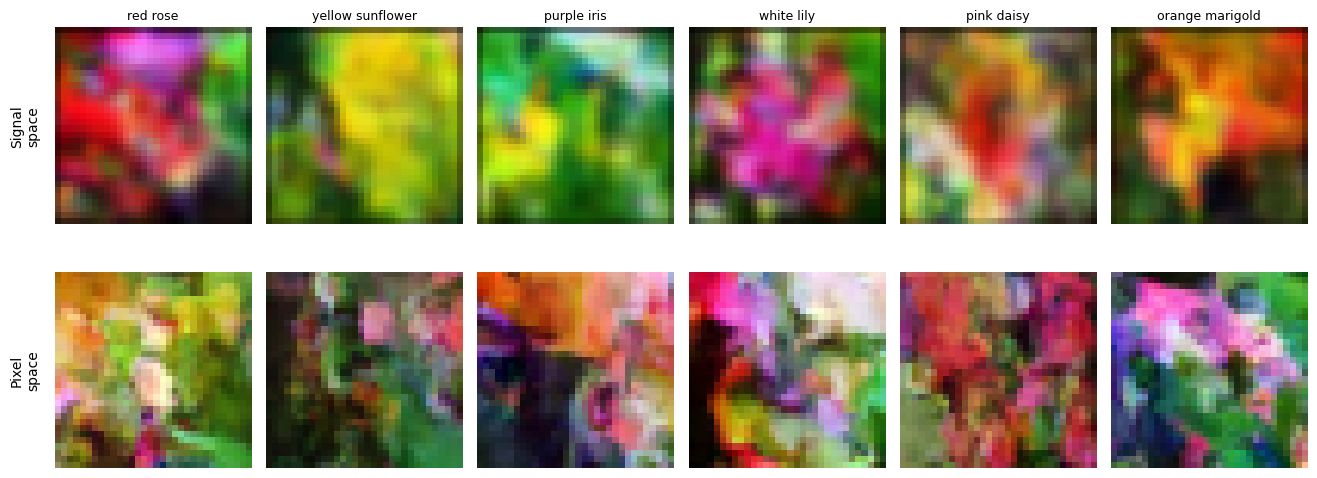
\includegraphics[width=\linewidth]{comparison_figure.png}
\caption{Random samples (temperature 1.0) from the best-checkpoint
  signal-space model (path only, 60~epochs, top row) and
  PixelCNN++ (60~epochs, bottom row) on six held-out text prompts.
  Both models were conditioned on the same CLIP ViT-B/32 embeddings.
  Oxford Flowers $32\times32$.}
\label{fig:samples}
\end{figure}

Two qualifications are in order. First, the signal-space model's
effective sequence is
\emph{longer} than the pixel-space model's by a factor of
$2 \cdot (1+f) \approx 2.16$, so per-step the comparison is less
unfavourable than it appears. Second, the path-encoding effect we
report is internal to the signal-space architecture and does not
generalise to pixel-space: PixelCNN++ has no separate ``path'' to
encode.

\subsection{Negative Results: CRT-Physics Modifications}\label{ssec:cnn}

To check that the path-encoding result is not an isolated
artefact within a broader ``CRT-inspired'' framing, we test three
additional modifications motivated by the analog physics of
cathode-ray tubes:
\textbf{P1, learned beam focus}: an auxiliary head emits a
per-step $\sigma_i \in [0.3, 1.5]$ which the renderer uses in place
of the fixed $\sigma$.
\textbf{P2, phosphor persistence}: a learnable convex combination
of the rendered image with a $3\times3$ blur of itself, initialised
at $10\%$ blur weight.
\textbf{P3, beam-position perturbation}: an auxiliary head emits
per-step $(\Delta x_i, \Delta y_i) \in [-0.5, 0.5]$ pixels added to
the canonical path position, with a small $\ell_2$ penalty on
$\Delta$.

Each modification is tested independently against a path-only
baseline at three seeds for ten epochs. \Cref{tab:postulates}
reports the result under a Welch $t$-test.

\begin{table}[t]
\centering
\caption{CRT-physics modifications vs.\ the path-only baseline on
Oxford Flowers $32\times32$, 10~epochs, 3~seeds. None reaches
significance.}
\label{tab:postulates}
\begin{tabular}{l S[table-format=5.1] S[table-format=4.1]
                  S[table-format=+4.1] S[table-format=+1.2]}
\toprule
& {NLL mean} & {NLL std} & {$\Delta$ vs.\ base} & {$t$} \\
\midrule
baseline (path only) & 17862.9 & 829.8 &      &  \\
\midrule
P1, learned $\sigma$ & 17472.4 & 185.6 & -390.5 & -0.80 \\
P2, persistence      & 17953.8 & 910.5 &  +90.9 & +0.13 \\
P3, beam perturb     & 17499.1 & 266.7 & -363.8 & -0.72 \\
\bottomrule
\end{tabular}
\end{table}

All three modifications produce $|t|<1$. We report this as a
meaningful negative result: the tested CRT-physics framing does not
generalise to additional architectural choices. The path-encoding
finding stands alone within this paper's design space.

% =====================================================================
\section{Extensions: Traversal Locality and Architectural Probes}%
\label{sec:extensions}

Two follow-up questions arise from the path-encoding result of
\cref{ssec:main}. First, if 2D path geometry matters, does the
\emph{choice} of 2D path matter among well-designed alternatives?
Second, can architectural modifications close the gap to
pixel-space methods? We answer each in turn -- both negatively
in absolute terms, but informatively about the underlying
bottleneck.

For this analysis we use $N{=}1024$ (single-sample-per-pixel
raster, no flyback) to enable a fair comparison across traversals
with the same sequence length. This differs from the V5 setup of
\cref{ssec:main} ($N{=}2208$, 2-spp + flyback); the two are not
directly comparable, and we report only same-$N$ deltas here.

\subsection{Locality Predicts bpd Across Traversals}%
\label{ssec:locality}

We define a traversal's \emph{locality} $\bar{\ell}(\mathcal{P})$
as the mean sequence distance between the four-neighbour pairs of
spatially adjacent pixels under path $\mathcal{P}$. We compare
four hand-designed traversals (raster, Hilbert, diagonal, spiral)
and five random pixel permutations, training each with the same
path-only configuration as \cref{ssec:main}.

% fig_locality.tex
% Scatter plot of traversal locality vs test bpd.
% Data from traversal_study.ipynb (Runs 1+2) and novel_arch_study.ipynb (Run 3).
% All points at N=1024, 30 epochs, path-only PE.

\begin{figure}[t]
\centering
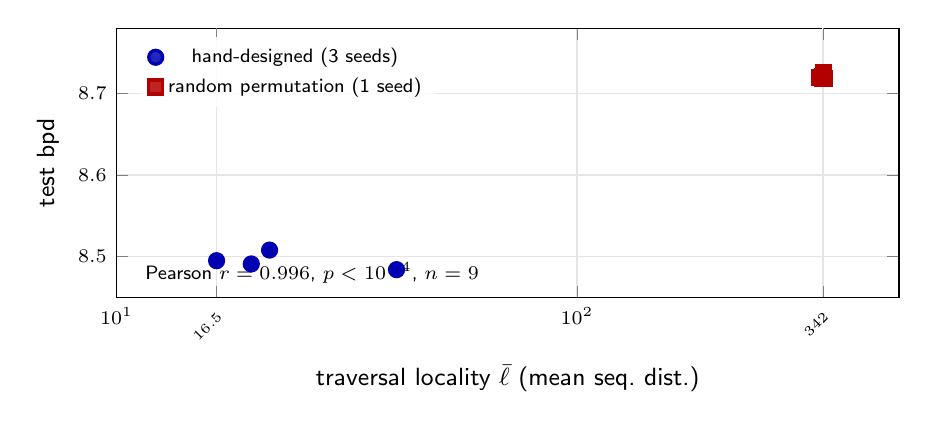
\begin{tikzpicture}
\begin{axis}[
    width=0.95\columnwidth,
    height=5cm,
    xlabel={traversal locality $\bar{\ell}$ (mean seq.\ dist.)},
    ylabel={test bpd},
    xmode=log,
    log basis x=10,
    xmin=10, xmax=500,
    ymin=8.45, ymax=8.78,
    xtick={10,100},
    extra x ticks={16.5,342},
    extra x tick labels={$16.5$,$342$},
    extra x tick style={tick label style={font=\sffamily\tiny,
                        rotate=45, anchor=north east}},
    grid=major,
    grid style={gray!20},
    legend pos=north west,
    legend style={font=\sffamily\scriptsize, draw=none,
                  fill=white, fill opacity=0.85, text opacity=1},
    label style={font=\sffamily\small},
    tick label style={font=\sffamily\scriptsize},
    every axis plot/.append style={very thick},
]

% hand-designed traversals (3 seeds each, mean bpd)
\addplot[only marks, mark=*, mark size=2.5pt, color=blue!70!black]
  coordinates {
    (16.5,  8.495)
    (19.625, 8.491)
    (21.5,  8.508)
    (40.5625, 8.484)
  };
\addlegendentry{hand-designed (3 seeds)}

% random pixel permutations (1 seed each)
\addplot[only marks, mark=square*, mark size=2.5pt, color=red!70!black]
  coordinates {
    (342.1, 8.7202)
    (341.3, 8.7189)
    (345.0, 8.7186)
    (342.3, 8.7254)
    (337.0, 8.7193)
  };
\addlegendentry{random permutation (1 seed)}

% Pearson r annotation
\node[font=\sffamily\scriptsize, anchor=south west]
  at (axis cs:11, 8.455)
  {Pearson $r=0.996$,\ $p<10^{-4}$,\ $n=9$};

\end{axis}
\end{tikzpicture}
\caption{Traversal locality $\bar{\ell}$ (mean sequence distance
  between four-neighbour pixel pairs) vs.\ test bpd on Oxford
  Flowers $32{\times}32$, $N{=}1024$, 30 epochs.
  Hand-designed paths (blue circles) cluster at
  $\bar{\ell}\in[16.5,\,40.6]$ and bpd $\in[8.48,\,8.51]$,
  which is statistically indistinguishable.
  Random pixel permutations (red squares) cluster at
  $\bar{\ell}\approx 342$ and bpd $\approx 8.72$.
  Across the full $20{\times}$ range the relationship is nearly
  linear in $\log\bar{\ell}$ (Pearson $r{=}0.996$,
  $p<10^{-4}$, $n{=}9$), identifying 1D-serialisation of 2D
  structure as the dominant bottleneck.}
\label{fig:locality}
\end{figure}


\Cref{tab:locality} reports test bpd alongside $\bar{\ell}$.
Within the hand-designed paths, bpd is statistically
indistinguishable: all four lie within $\pm0.013$~bpd, well
inside seed noise. Across the full range of $\bar{\ell}$ -- from
$16.5$ (raster) to $\approx 342$ (random permutations) -- bpd
grows almost linearly with $\bar{\ell}$, with Pearson $r{=}0.996$
($p<10^{-4}$, $n{=}9$; \cref{fig:locality}). Locality is
therefore \emph{not} predictive among well-designed paths, but is
a remarkably tight predictor across the full range, locating the
bottleneck in 1D serialisation of 2D-neighbour structure rather
than the specific choice of scan order.

\begin{table}[t]
\centering
\caption{Traversal locality vs.\ test bpd at $N{=}1024$, 30
  epochs. Hand-designed paths use 3 seeds; random paths use 1 seed
  each. Lower bpd is better.}
\label{tab:locality}
\begin{tabular}{l S[table-format=3.1] S[table-format=1.3(3)]}
\toprule
Traversal & {$\bar{\ell}$} & {bpd (test)} \\
\midrule
raster ($N{=}1024$)  & 16.5  & 8.495(23) \\
Hilbert              & 19.6  & 8.491(23) \\
diagonal             & 21.5  & 8.508(22) \\
spiral               & 40.6  & 8.484(24) \\
\midrule
random $r_0$         & 342.1 & {8.720} \\
random $r_1$         & 341.3 & {8.719} \\
random $r_2$         & 345.0 & {8.719} \\
random $r_3$         & 342.3 & {8.725} \\
random $r_4$         & 337.0 & {8.719} \\
\midrule
\multicolumn{3}{l}{Pearson $r = 0.996$,\ $p<10^{-4}$,\ $n{=}9$} \\
\bottomrule
\end{tabular}
\end{table}

\subsection{Architectural Probes Do Not Close the Gap}%
\label{ssec:probes}

Motivated by the locality finding, we test four interventions
designed either to improve locality (patch-hierarchical
traversal), to inject local inductive bias along the sequence
(causal 1D conv-stem), to diversify the scan-order seen during
training (epoch-level traversal augmentation), or to
re-parameterise the predictive target (delta input encoding).
\Cref{tab:probes} reports bpd against the matched-$N$ raster
baseline (\SI{8.495}{} bpd, 3 seeds).

\begin{table}[t]
\centering
\caption{Architectural probes against the raster baseline at
  $N{=}1024$, 30 epochs. None improves over baseline; the
  conv-stem seed-0 run triggered an early-abort gate
  (seed-0 bpd $> \text{baseline} + 0.30$).}
\label{tab:probes}
\begin{tabular}{l S[table-format=1.3(3)] S[table-format=+1.3]
                S[table-format=1]}
\toprule
Variant & {bpd mean} & {$\Delta$ baseline} & {seeds} \\
\midrule
raster baseline                   & 8.495(23) & {---}  & 3 \\
delta input encoding              & 8.768(14) & +0.273 & 3 \\
patch-hierarchical ($8{\times}8$) & 8.512(22) & +0.017 & 3 \\
traversal augmentation            & 8.505(26) & +0.010 & 3 \\
causal 1D conv-stem               & {8.799}   & +0.304 & 1 \\
\bottomrule
\end{tabular}
\end{table}

None of the four probes improves over the baseline. Three
(patch-hierarchical, traversal augmentation, delta encoding) lie
within or just outside seed noise and may be benign re-orderings
of the same problem; the conv-stem is worse by $0.30$~bpd,
sufficient to trigger early abort. We read these results as
narrowing the design space: short-range temporal aggregation by a
causal 1D conv-stem is the wrong inductive bias (the bottleneck
demands 2D-neighbour aggregation), and surface-level reorderings
of the path do not alter the underlying 1D-serialisation problem
identified in \cref{ssec:locality}. The remaining gap to
pixel-space methods most likely requires either a 2D-aware
computational block (e.g.\ local 2D-window attention with
appropriate causal masking, or a patch-level transformer with
intra-patch and inter-patch attention) or a fundamentally
different output factorisation. We leave both directions to
future work.

% =====================================================================
\section{Discussion}\label{sec:discussion}

\paragraph{Why does the sequence encoding hurt?}
Both sinusoidal encodings carry the same Shannon information about
position: the path is invertible, so the sequence index and the
2D coordinate determine each other. The two encodings differ in
\emph{geometry}: the sequence encoding lays positions on a single
1D line, while the path encoding lays them on a folded 2D
trajectory whose neighbours in path space are also neighbours in
sequence space, but whose far-apart points in path space can be
near-neighbours in 2D after the row wraps. We conjecture (without
proving) that adding both encodings creates competing gradient
signals on a shared embedding subspace and slows the optimiser
without providing additional information. A more careful study of
the learned embeddings in each configuration is left to future work.

\paragraph{Why doesn't this close the gap to PixelCNN++?}
Pixel-space autoregressive models exploit local 2D conditional
structure directly through their masked convolutions. The
signal-space model has to recover this structure through a
1D causal attention over a sequence that visits 2D-neighbours
across long sequence distances (one full row apart). Even with the
correct positional encoding, this is a harder optimisation problem
for the same parameter budget. We tested four candidate interventions in \cref{ssec:probes} --
including a patch-hierarchical scan inspired by space-filling
curves~\cite{li2025direction,li2025radar} -- and none improved
over the matched-$N$ baseline. Combined with the locality finding
of \cref{ssec:locality}, this points specifically to 2D-aware
intermediate computations (rather than further scan-order
exploration) as the remaining lever; we leave that to future work.

\paragraph{Limitations.}
(i) All experiments are on a single dataset (Oxford Flowers~102) at
small resolutions. Generalisation to natural-image distributions
such as CIFAR-10 or LSUN is not tested.
(ii) The $48\times48$ scaling result shows the correct direction
but with Welch $t=-1.97$, weaker than the $32\times32$ result
($t=5.4$), due to high cross-seed variance; one seed achieved
unusually low loss while the others converged to a different basin.
(iii) The transformer's $O(N^2)$ attention prevents experiments at
$\geq 64\times 64$ in our compute budget without architectural
changes such as KV caching or sparse attention.
(iv) The PixelCNN++ implementation uses a single causal stack rather
than the original's dual horizontal-and-vertical stacks; published
PixelCNN++ numbers on CIFAR-10 (\SI{2.92}{} bpd) are therefore not
directly attainable in our setup.

% =====================================================================
\section{Conclusion}

In raster-scan signal-space autoregressive image generation, an
explicit 2D path positional encoding makes the standard 1D sequence
encoding redundant, and adding both reliably degrades test
likelihood. Three CRT-physics--motivated modifications failed to
produce significant gains, suggesting that the encoding effect is
specific rather than a symptom of broader architectural under-fit.
A matched-parameter PixelCNN++ retains an absolute likelihood
advantage on the same data, framing our finding as a clean ablation
result within signal-space autoregressive models rather than a
challenge to pixel-space methods.
Extending these results, traversal locality predicts test bpd with
Pearson $r=0.996$ ($p<10^{-4}$, $n{=}9$) across hand-designed and
random paths at matched $N{=}1024$, and four architectural probes
(delta input encoding, patch-hierarchical traversal, traversal
augmentation, causal 1D conv-stem) all fail to improve over that
baseline, locating the remaining gap to pixel-space methods in
2D-aware computation rather than scan-order choice.

% =====================================================================
\section*{Acknowledgements}

The authors thank the MechaML reading group for early feedback on
the signal-space framing. Compute was provided by Kaggle Notebooks
and Google Colab free tiers; we are grateful for these resources.

% =====================================================================
\begin{thebibliography}{00}

\bibitem{vandenoord2016pixelrnn}
A. van den Oord, N. Kalchbrenner, and K. Kavukcuoglu,
``Pixel recurrent neural networks,''
in \textit{Proc. Int. Conf. Mach. Learn. (ICML)}, 2016, pp.~1747--1756.

\bibitem{salimans2017pixelcnnpp}
T. Salimans, A. Karpathy, X. Chen, and D. P. Kingma,
``PixelCNN++: Improving the PixelCNN with discretized logistic mixture
likelihood and other modifications,''
in \textit{Proc. Int. Conf. Learn. Represent. (ICLR)}, 2017.

\bibitem{parmar2018imagetransformer}
N. Parmar \textit{et al.},
``Image transformer,''
in \textit{Proc. Int. Conf. Mach. Learn. (ICML)}, 2018, pp.~4055--4064.

\bibitem{chen2020generative}
M. Chen \textit{et al.},
``Generative pretraining from pixels,''
in \textit{Proc. Int. Conf. Mach. Learn. (ICML)}, 2020, pp.~1691--1703.

\bibitem{ha2017sketchrnn}
D. Ha and D. Eck,
``A neural representation of sketch drawings,''
in \textit{Proc. Int. Conf. Learn. Represent. (ICLR)}, 2018.

\bibitem{ganin2018spiral}
Y. Ganin, T. Kulkarni, I. Babuschkin, S. M. A. Eslami, and O. Vinyals,
``Synthesizing programs for images using reinforced adversarial
learning,''
in \textit{Proc. Int. Conf. Mach. Learn. (ICML)}, 2018, pp.~1666--1675.

\bibitem{liu2021painttransformer}
S. Liu \textit{et al.},
``Paint transformer: Feed forward neural painting with stroke
prediction,''
in \textit{Proc. IEEE/CVF Int. Conf. Comput. Vis. (ICCV)}, 2021,
pp.~6598--6607.

\bibitem{frans2021clipdraw}
K. Frans, L. B. Soros, and O. Witkowski,
``CLIPDraw: Exploring text-to-drawing synthesis through language-image
encoders,''
in \textit{Adv. Neural Inf. Process. Syst. (NeurIPS)}, 2022.

\bibitem{jain2023vectorfusion}
A. Jain, A. Xie, and P. Abbeel,
``VectorFusion: Text-to-SVG by abstracting pixel-based diffusion
models,''
in \textit{Proc. IEEE/CVF Conf. Comput. Vis. Pattern Recognit. (CVPR)},
2023, pp.~1911--1920.

\bibitem{li2020diffvg}
T.-M. Li, M. Luk{\'a}{\v c}, M. Gharbi, and J. Ragan-Kelley,
``Differentiable vector graphics rasterization for editing and
learning,''
\textit{ACM Trans. Graph.}, vol.~39, no.~6, pp.~1--15, 2020.

\bibitem{kerbl20233dgaussian}
B. Kerbl, G. Kopanas, T. Leimk{\"u}hler, and G. Drettakis,
``3D Gaussian splatting for real-time radiance field rendering,''
\textit{ACM Trans. Graph.}, vol.~42, no.~4, pp.~1--14, 2023.

\bibitem{li2025radar}
Z. Li \textit{et al.},
``RadAR: Radial autoregressive image generation,''
\textit{arXiv preprint arXiv:2512.24639}, 2025.

\bibitem{li2025direction}
Y. Li \textit{et al.},
``Direction-aware diagonal autoregressive image generation,''
\textit{arXiv preprint arXiv:2503.11129}, 2025.

\bibitem{perez2018film}
E. Perez, F. Strub, H. de Vries, V. Dumoulin, and A. C. Courville,
``FiLM: Visual reasoning with a general conditioning layer,''
in \textit{Proc. AAAI Conf. Artif. Intell.}, 2018, pp.~3942--3951.

\bibitem{vaswani2017attention}
A. Vaswani \textit{et al.},
``Attention is all you need,''
in \textit{Adv. Neural Inf. Process. Syst. (NIPS)}, 2017, pp.~5998--6008.

\bibitem{nilsback2008flowers}
M.-E. Nilsback and A. Zisserman,
``Automated flower classification over a large number of classes,''
in \textit{Proc. Indian Conf. Comput. Vis. Graph. Image Process.}, 2008,
pp.~722--729.

\bibitem{bengio2015scheduled}
S. Bengio, O. Vinyals, N. Jaitly, and N. Shazeer,
``Scheduled sampling for sequence prediction with recurrent neural
networks,''
in \textit{Adv. Neural Inf. Process. Syst. (NIPS)}, 2015, pp.~1171--1179.

\bibitem{loshchilov2019adamw}
I. Loshchilov and F. Hutter,
``Decoupled weight decay regularization,''
in \textit{Proc. Int. Conf. Learn. Represent. (ICLR)}, 2019.

\end{thebibliography}

\end{document}
